\chapter{Michelson Interferometer}

\begin{figure}[htbp]
    \centering
    \begin{tikzpicture}[
        scale=1.0,
        beam/.style={thick, draw=black!80},
        fwd/.style={
            postaction={
                decorate,
                decoration={
                    markings,
                    mark=at position #1 with {\arrow{Stealth[length=2mm, width=1.5mm]}}
                }
            }
        },
        rev/.style={
            postaction={
                decorate,
                decoration={
                    markings,
                    mark=at position #1 with {\arrow{Stealth[length=2mm, width=1.5mm, reversed]}}
                }
            }
        }
    ]
        % ==========================================
        % Source plane S (Left)
        % ==========================================
        \draw[very thick, black!85] (-3.2, -1.1) -- (-3.2, 1.1);
        \node[above, font=\small] at (-3.2, 1.15) {$S$};

        % ==========================================
        % Beam Splitter BS (Center, tilted at 45 deg)
        % Top edge passes through beam intersection (0,0)
        % ==========================================
        \begin{scope}[shift={(0,0)}, rotate=45]
            \draw[very thick, fill=gray!15, draw=black!85] (-1.05, -0.28) rectangle (1.05, 0);
        \end{scope}
        \node[above right, font=\small] at (0.75, 0.65) {BS};

        % ==========================================
        % Mirror M2 (Top)
        % ==========================================
        \draw[very thick, fill=gray!25, draw=black!85] (-0.75, 3.35) rectangle (0.75, 3.65);
        \node[above, font=\small] at (0, 3.7) {$M2$};

        % ==========================================
        % Mirror M1 (Right)
        % ==========================================
        \draw[very thick, fill=gray!25, draw=black!85] (3.35, -0.75) rectangle (3.65, 0.75);
        \node[below, font=\small] at (3.5, -0.85) {$M1$};

        % ==========================================
        % Beam (1): Source S to Beam Splitter BS
        % ==========================================
        \draw[beam, fwd=0.55] (-3.2, 0) -- (0, 0);
        \node[above, font=\small] at (-1.6, 0.1) {$(1)$};

        % ==========================================
        % Beam (2): BS up to M2 and back
        % ==========================================
        \draw[beam, fwd=0.55, rev=0.75] (0, 0) -- (0, 3.35);
        \node[right, font=\small] at (0.12, 1.55) {$(2)$};

        % ==========================================
        % Beam (3): BS right to M1 and back
        % ==========================================
        \draw[beam, fwd=0.55, rev=0.75] (0, 0) -- (3.35, 0);
        \node[above, font=\small] at (1.75, 0.12) {$(3)$};

        % ==========================================
        % Beam (4): Recombined output downward
        % ==========================================
        \draw[beam, fwd=0.55] (0, 0) -- (0, -2.5);
        \node[right, font=\small] at (0.12, -1.45) {$(4)$};

        % Sub-label (a)
        \node[below, font=\small] at (0, -2.65) {(a)};
    \end{tikzpicture}
    \caption{Schematic of the Michelson interferometer, \cite[Chap 8.]{pedrottiIntroductionOptics2007}.}
    \label{fig:schematic_michelson_interferometer}
\end{figure}

A schematic of the michelson interferometer is shown in \cref{fig:schematic_michelson_interferometer}, from the source of light (S) we get the beam (1) being split by the beam splitter (BS) resulting in beams (3) transmitted and (2) by reflection, these reflect on mirrors (M1) and (M2) respectively and return to the BS where (3) is reflected and (2) is transmitted, and the two beams come together exiting the interferometer as beam (4). Thus, beam 4 includes rays that have traveled different optical paths and will demonstrate interference \cite[Chap 8.]{pedrottiIntroductionOptics2007}.



\begin{figure}[htbp]
    \centering
    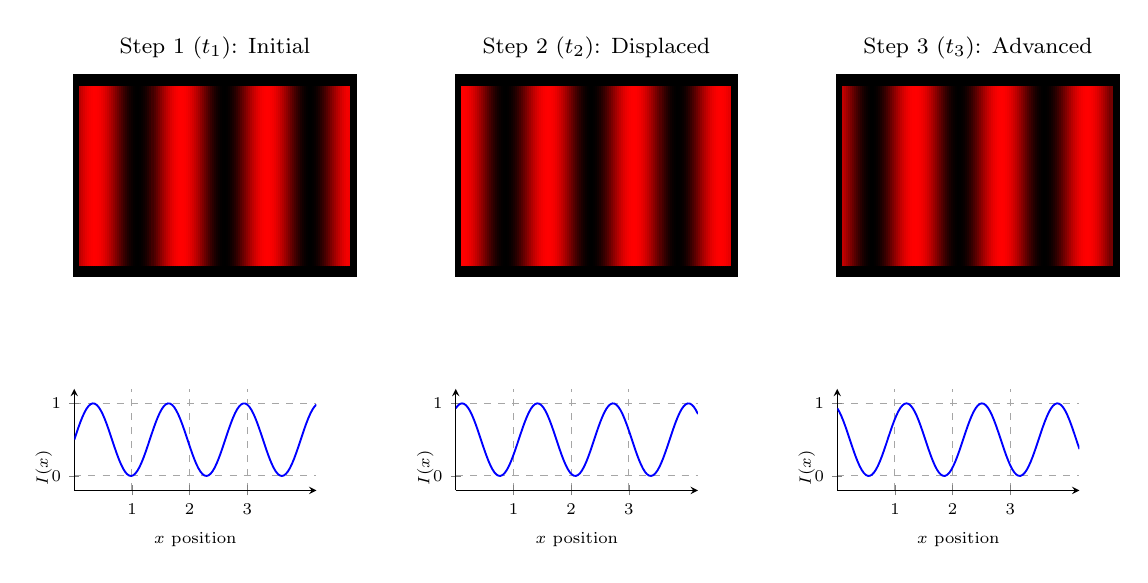
\begin{tikzpicture}[scale=0.85]
        % ==========================================
        % STEP 1: t_1 (Initial Position)
        % ==========================================
        \begin{scope}[shift={(0,0)}]
            % Camera View Box (Denser fringes for smooth gradient)
            \draw[thick, fill=black] (0,3.2) rectangle (4.2,6.2);
            \node[above, font=\footnotesize] at (2.1,6.3) {Step 1 ($t_1$): Initial};
            \foreach \x in {0.10, 0.13, ..., 4.10} {
                \pgfmathsetmacro{\intensity}{sin(\x * 280)*50 + 50}
                \draw[color=red!\intensity!black, line width=0.45mm] (\x, 3.35) -- (\x, 6.05);
            }
            \draw[thick] (0,3.2) rectangle (4.2,6.2);

            % Intensity Plot (Enlarged width and height)
            \begin{axis}[
                at={(0,0)},
                anchor=south west,
                width=5.2cm,
                height=3.1cm,
                xmin=0, xmax=4.2,
                ymin=-0.2, ymax=1.2,
                axis lines=left,
                xlabel={$x$ position},
                ylabel={$I(x)$},
                font=\scriptsize,
                xtick={1, 2, 3},
                ytick={0,1},
                grid=major,
                grid style={dashed, gray!70},
                xlabel style={below=1pt},
                ylabel style={left=1pt}
            ]
                \addplot[domain=0:4.2, samples=120, thick, blue] {sin(deg(x*4.8))*0.5 + 0.5};
            \end{axis}
        \end{scope}

        % ==========================================
        % STEP 2: t_2 (Intermediate Displacement)
        % ==========================================
        \begin{scope}[shift={(5.7,0)}]
            % Camera View Box
            \draw[thick, fill=black] (0,3.2) rectangle (4.2,6.2);
            \node[above, font=\footnotesize] at (2.1,6.3) {Step 2 ($t_2$): Displaced};
            \foreach \x in {0.10, 0.13, ..., 4.10} {
                \pgfmathsetmacro{\intensity}{sin(\x * 280 + 60)*50 + 50}
                \draw[color=red!\intensity!black, line width=0.45mm] (\x, 3.35) -- (\x, 6.05);
            }
            \draw[thick] (0,3.2) rectangle (4.2,6.2);

            % Intensity Plot (Enlarged width and height)
            \begin{axis}[
                at={(0,0)},
                anchor=south west,
                width=5.2cm,
                height=3.1cm,
                xmin=0, xmax=4.2,
                ymin=-0.2, ymax=1.2,
                axis lines=left,
                xlabel={$x$ position},
                ylabel={$I(x)$},
                font=\scriptsize,
                xtick={1, 2, 3},
                ytick={0,1},
                grid=major,
                grid style={dashed, gray!70},
                xlabel style={below=1pt},
                ylabel style={left=1pt}
            ]
                \addplot[domain=0:4.2, samples=120, thick, blue] {sin(deg(x*4.8) + 60)*0.5 + 0.5};
            \end{axis}
        \end{scope}

        % ==========================================
        % STEP 3: t_3 (Advanced Displacement)
        % ==========================================
        \begin{scope}[shift={(11.4,0)}]
            % Camera View Box
            \draw[thick, fill=black] (0,3.2) rectangle (4.2,6.2);
            \node[above, font=\footnotesize] at (2.1,6.3) {Step 3 ($t_3$): Advanced};
            \foreach \x in {0.10, 0.13, ..., 4.10} {
                \pgfmathsetmacro{\intensity}{sin(\x * 280 + 120)*50 + 50}
                \draw[color=red!\intensity!black, line width=0.45mm] (\x, 3.35) -- (\x, 6.05);
            }
            \draw[thick] (0,3.2) rectangle (4.2,6.2);

            % Intensity Plot (Enlarged width and height)
            \begin{axis}[
                at={(0,0)},
                anchor=south west,
                width=5.2cm,
                height=3.1cm,
                xmin=0, xmax=4.2,
                ymin=-0.2, ymax=1.2,
                axis lines=left,
                xlabel={$x$ position},
                ylabel={$I(x)$},
                font=\scriptsize,
                xtick={1, 2, 3},
                ytick={0,1},
                grid=major,
                grid style={dashed, gray!70},
                xlabel style={below=1pt},
                ylabel style={left=1pt}
            ]
                \addplot[domain=0:4.2, samples=120, thick, blue] {sin(deg(x*4.8) + 120)*0.5 + 0.5};
            \end{axis}
        \end{scope}

    \end{tikzpicture}
    \caption{Sequential time-steps illustrating high-density fringe gradients captured by the camera sensor and the corresponding phase translation of peaks in the 1D intensity profile $I(x)$ during mirror displacement.}
    \label{fig:three_step_fringes}
\end{figure}

\section{Interferometer Design and Hardware Configuration}

\begin{figure}[htbp]
    \centering
    \begin{subfigure}{0.45\textwidth}
        \centering
        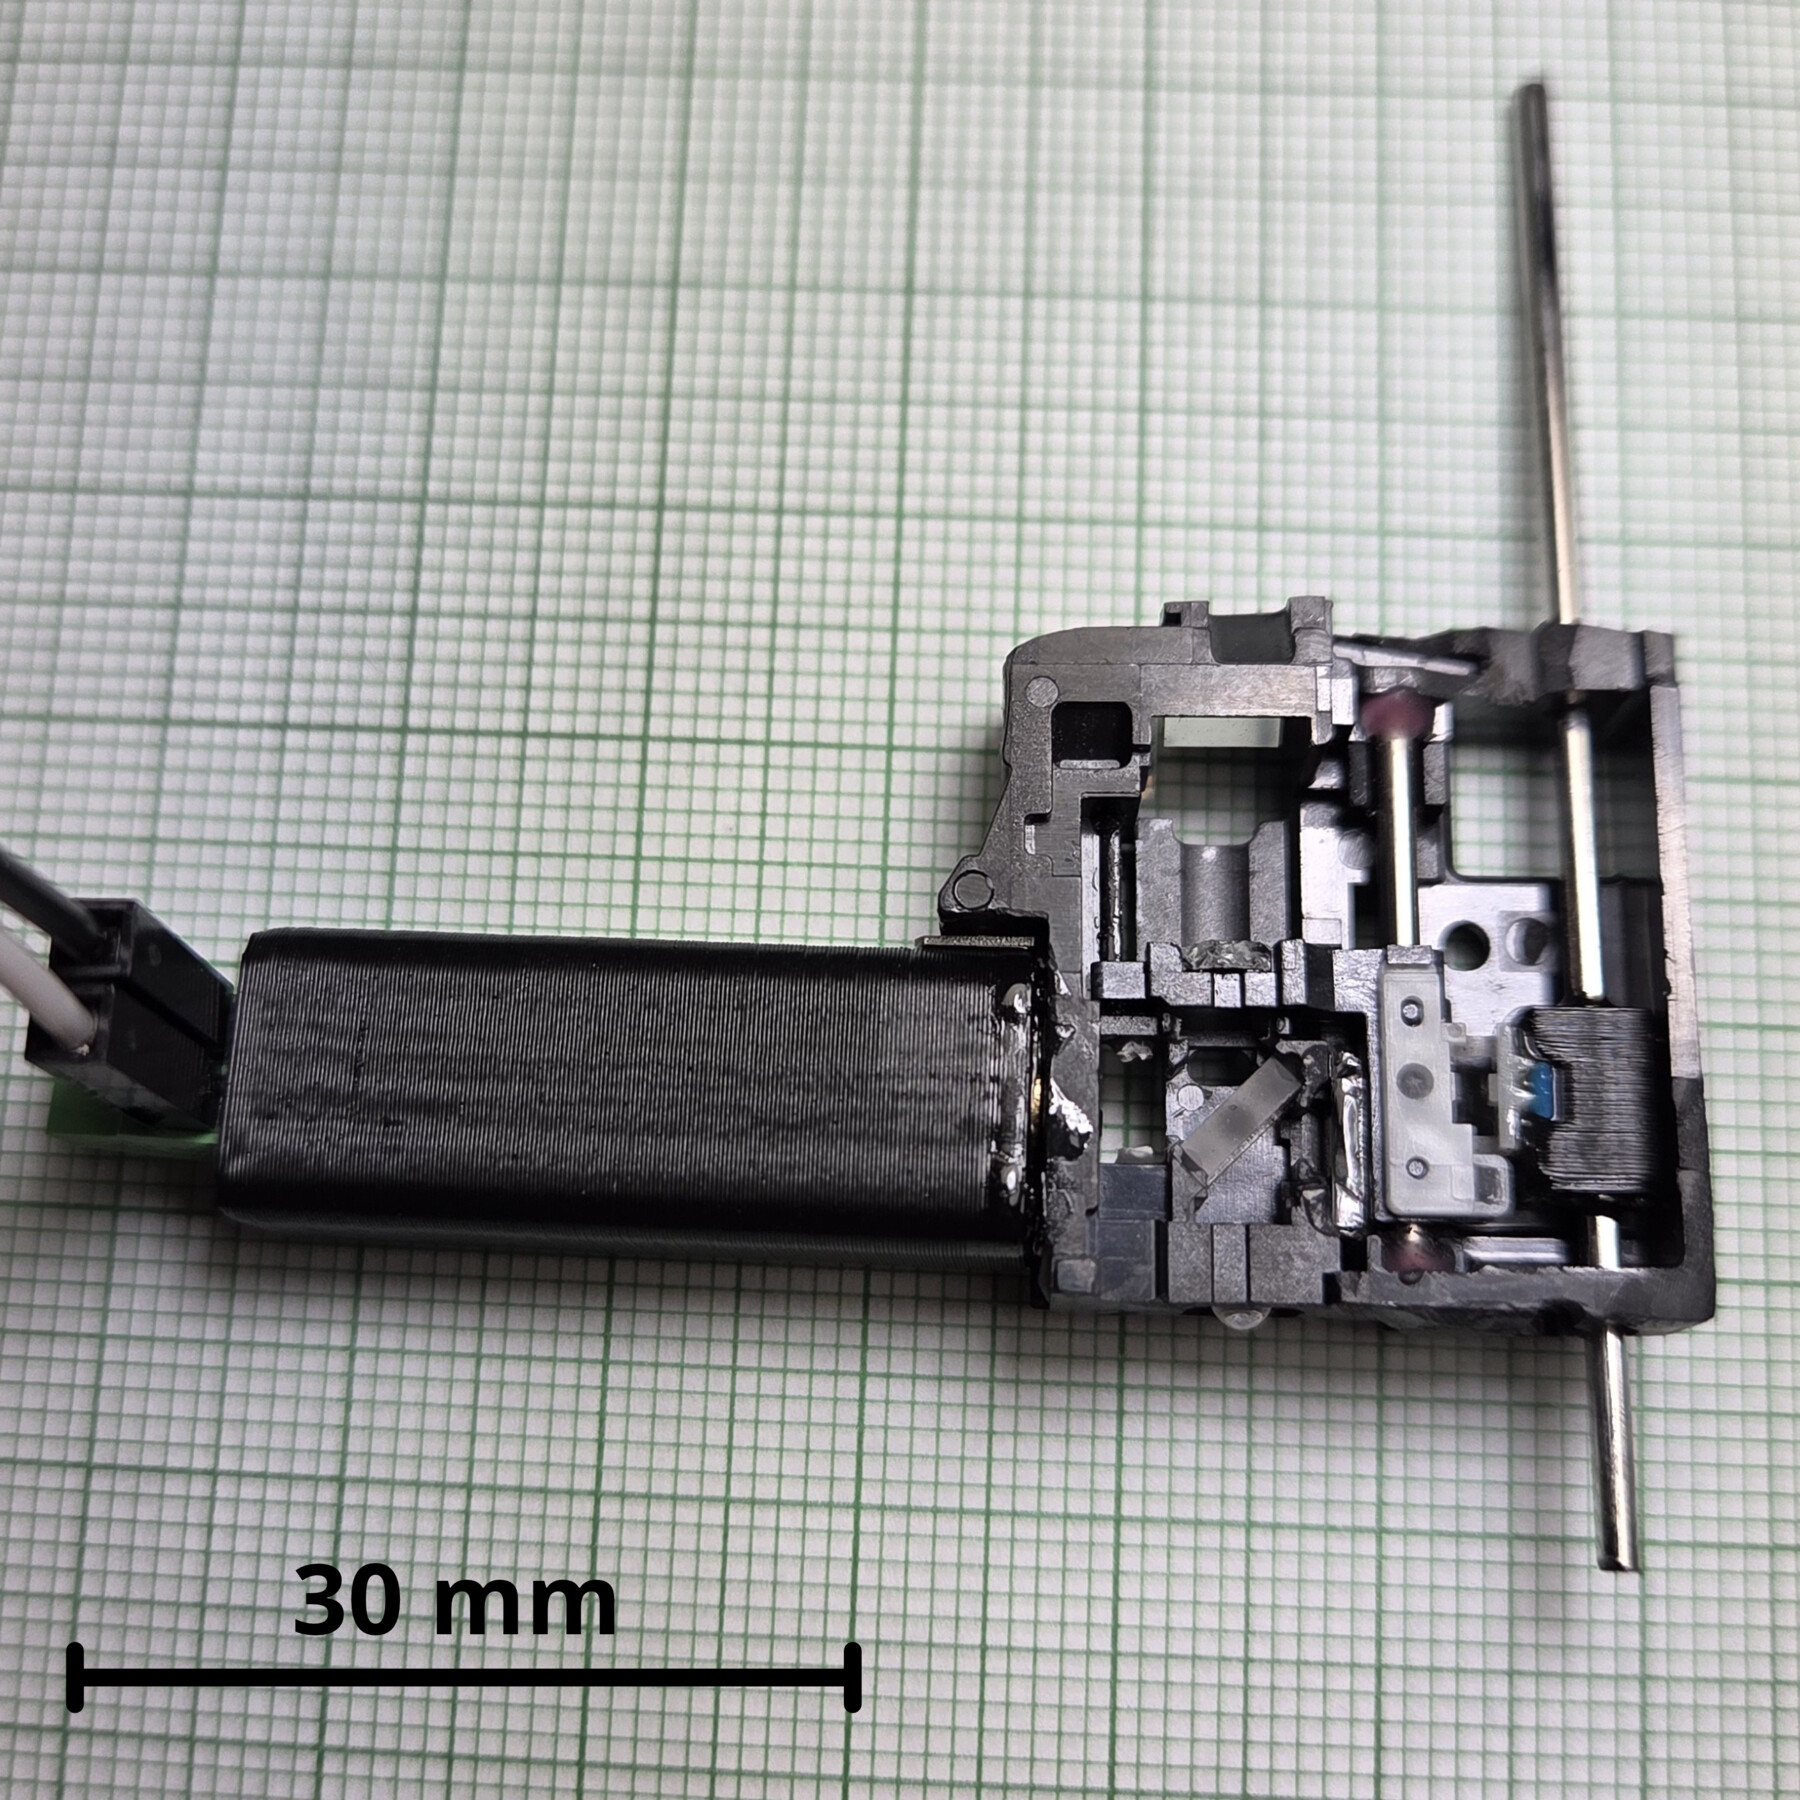
\includegraphics[width=\textwidth]{images/interferometer_top_big_compressed.jpg}
        \caption{Interferometer}
        \label{fig:interferometer_top}
    \end{subfigure}\hfill
    \begin{subfigure}{0.45\textwidth}
        \centering
        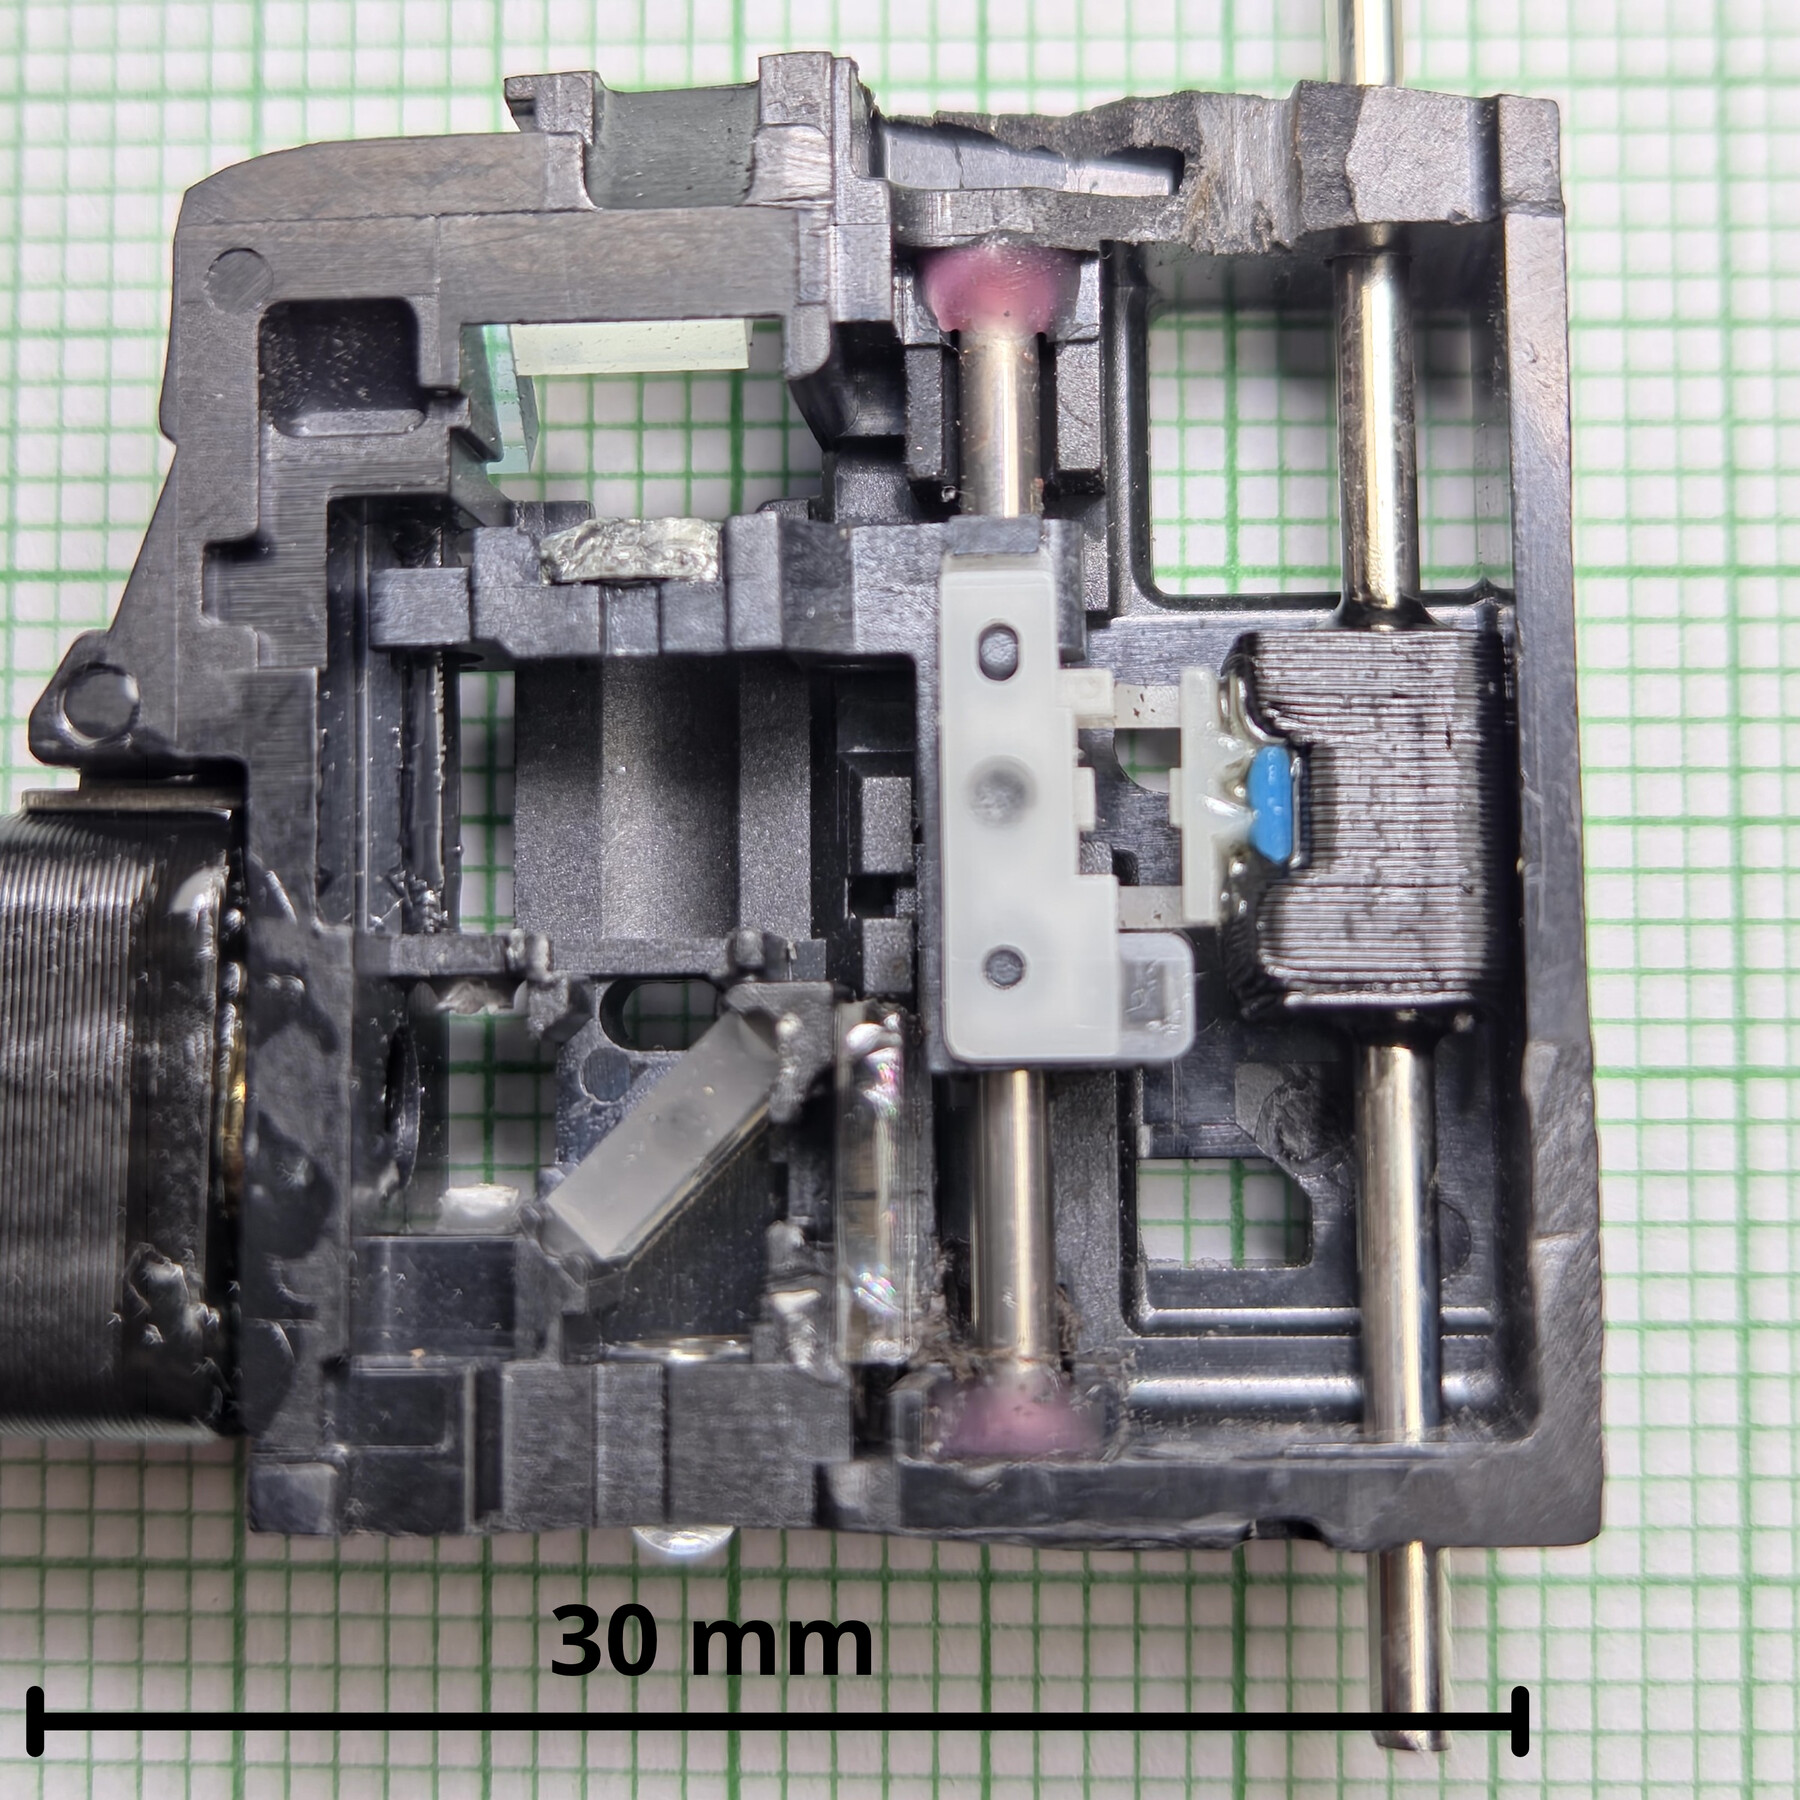
\includegraphics[width=\textwidth]{images/interferometer_top_zoomed_test.jpg}
        \caption{Interferometer (Zoomed)}
        \label{fig:interferometer_top_zoomed}
    \end{subfigure}
    \caption{Interferometer Experimental Setup. a) Top view; b) Zoomed top view with details of the mirrors and axis mounting.}
    \label{fig:interferometer_setup}
\end{figure}


In the \cref{fig:interferometer_setup} we can see the top view of the  interferometer constructed as shown in the figure, the interferometer is compact and robust, with a design that minimizes vibrations and misalignments by using a rigid casing and keeping the optical components close together, this creates a stable optical path and reduces the impact of external disturbances due to the vibrations of the system as a whole. The compactness of the device also allows for easier alignment of the optical components, as the distances between them are small, reducing the chances of misalignment when the shafts transfer the actuator motion into the movable mirror, the thermal expansion effects are also reduced due to uniform heat conduction between the components because of their proximity, improving the overall performance of the interferometer. The design compactness also allows for easy coupling to other systems and can be integrated into larger experimental setups without taking up much space, making it suitable for applications where space is limited.

\begin{figure}[htbp]
    \centering
    \begin{subfigure}{0.45\textwidth}
        \centering
        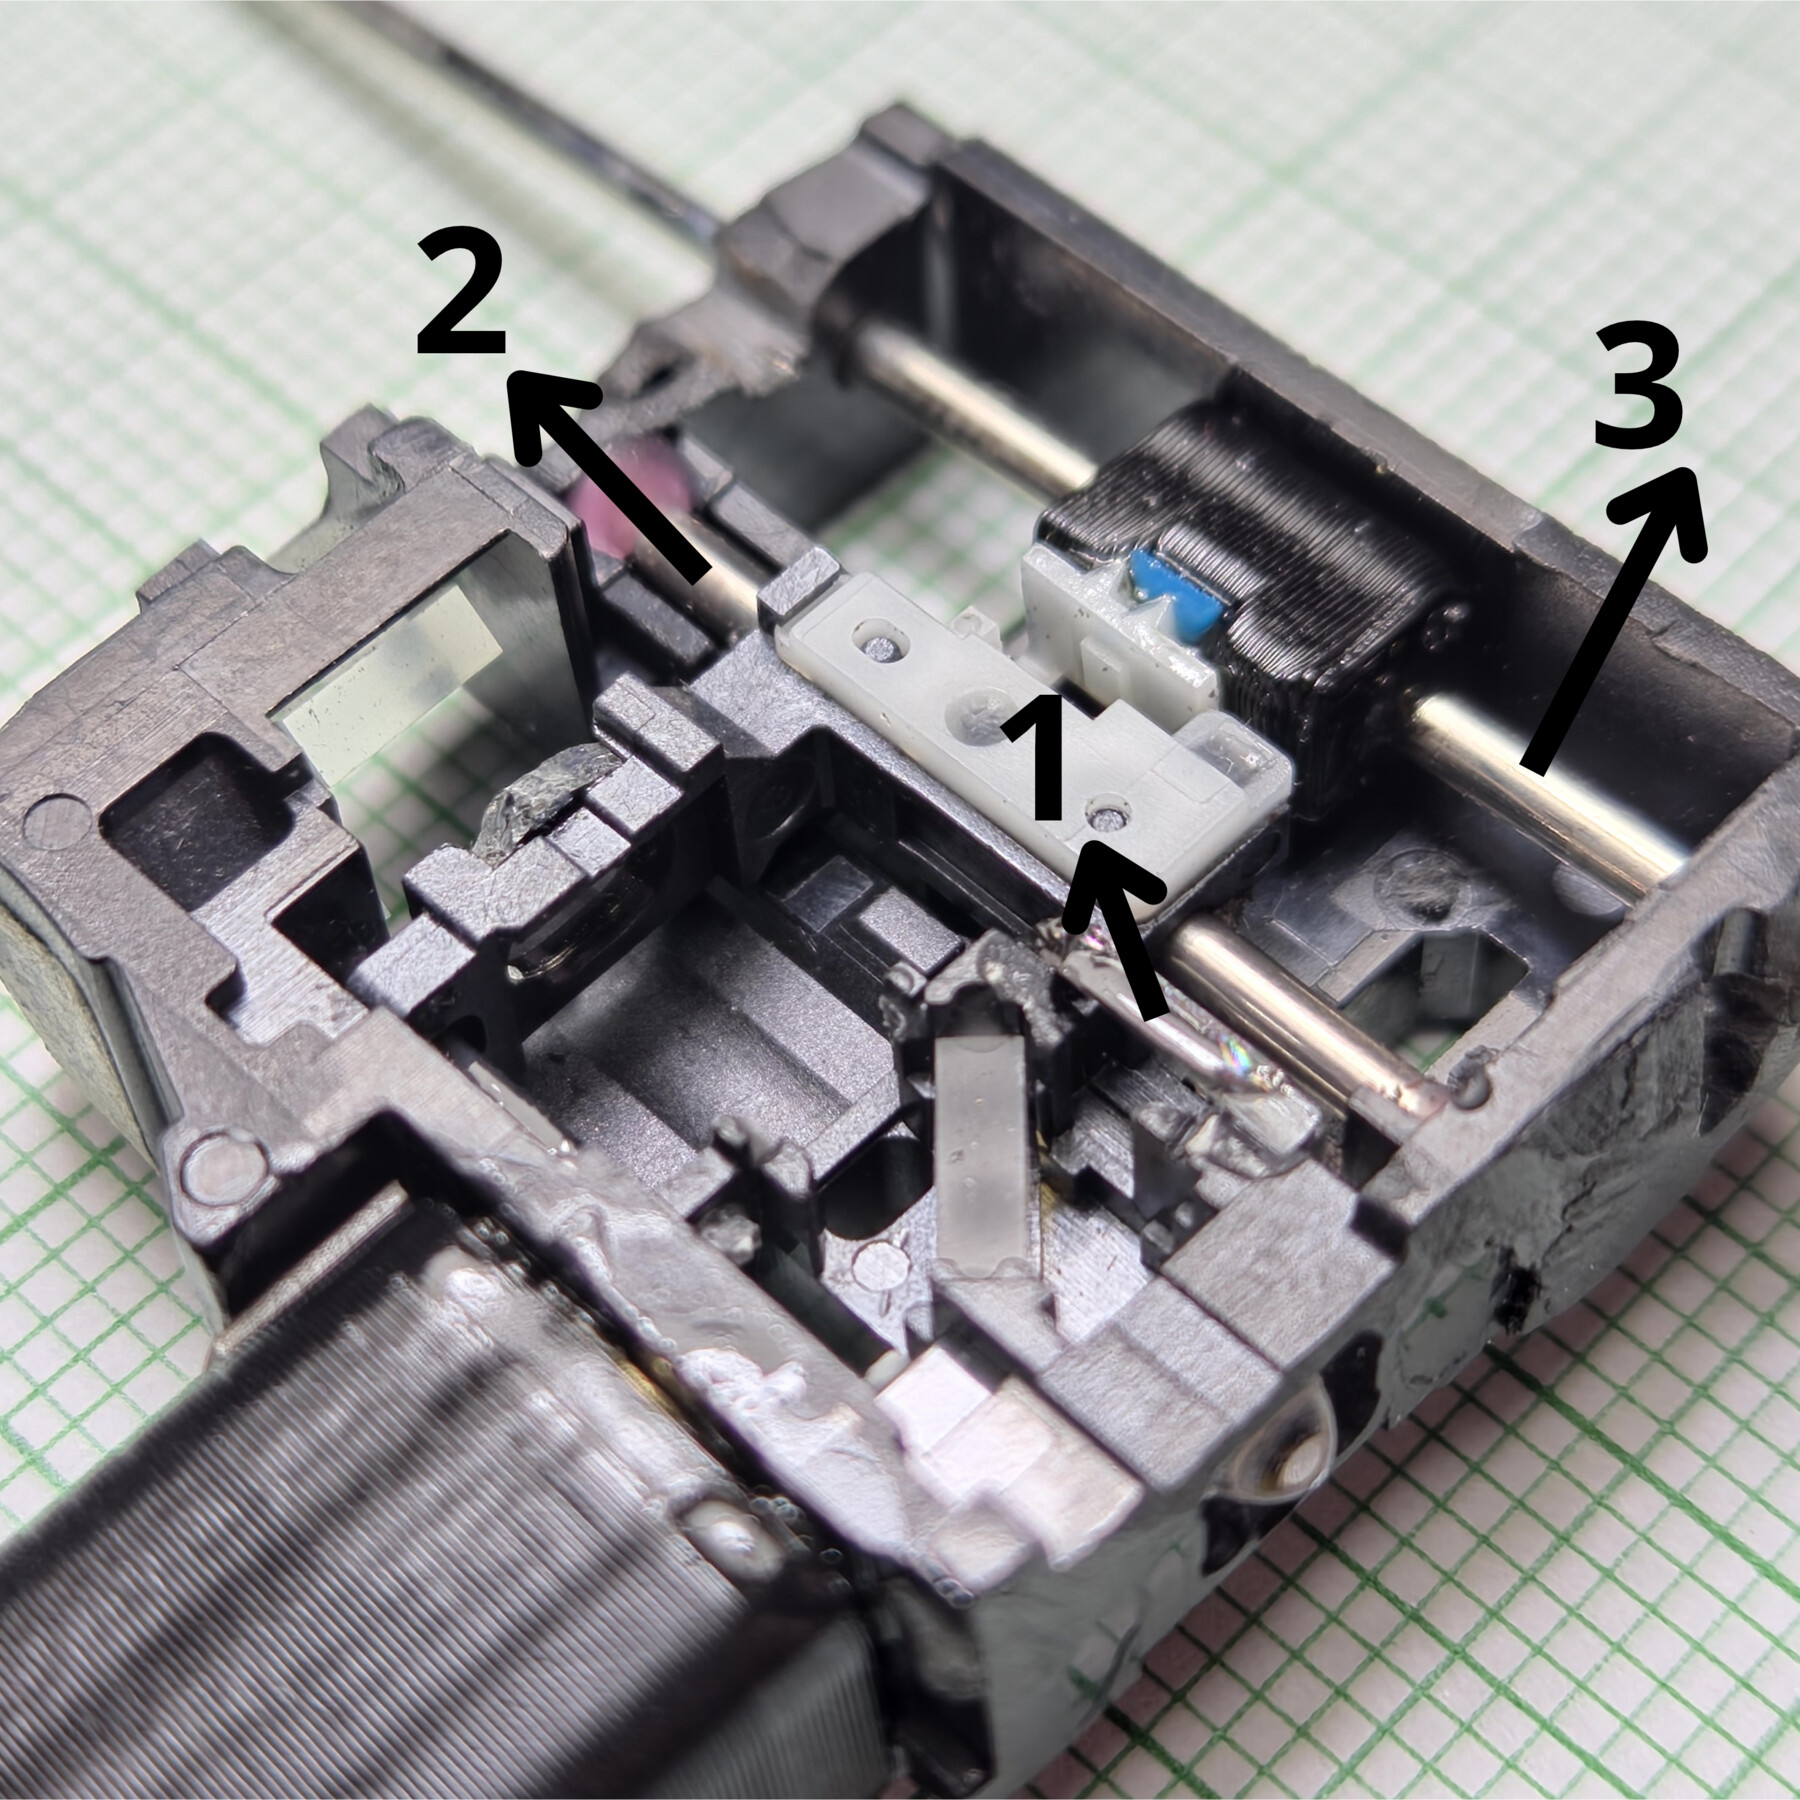
\includegraphics[width=\textwidth]{images/interferometer_side_compressed.jpg}
        \caption{Interferometer side view}
        \label{fig:interferometer_side_a}
    \end{subfigure}\hfill
    \begin{subfigure}{0.45\textwidth}
        \centering
        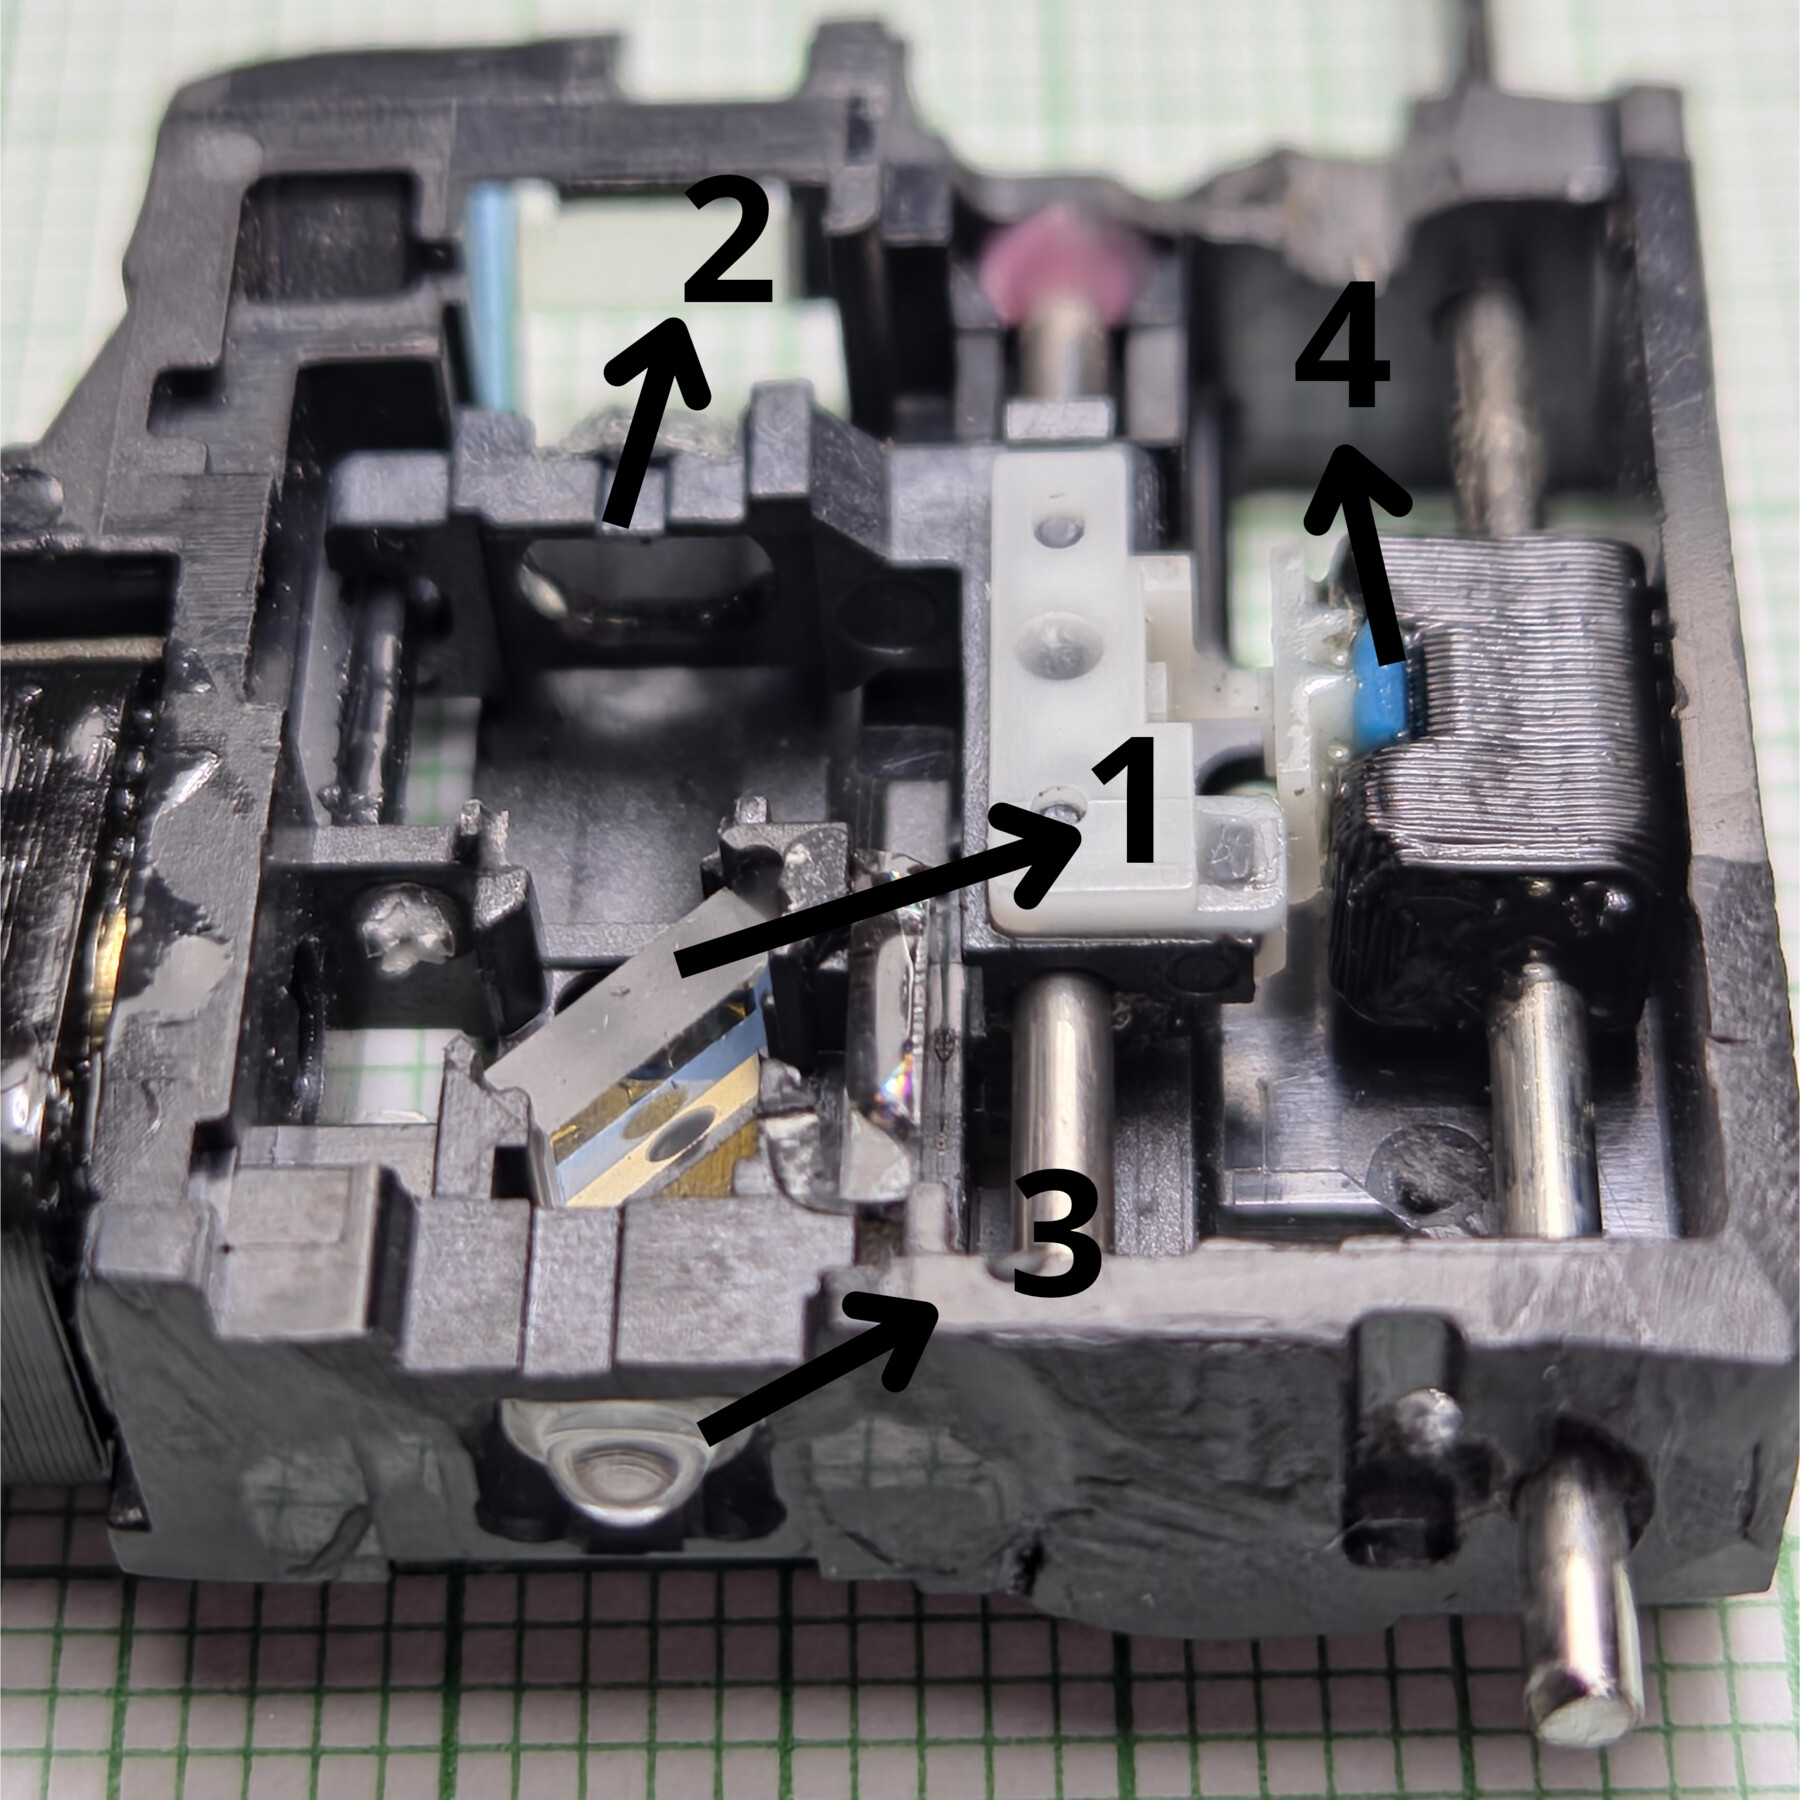
\includegraphics[width=\textwidth]{images/interferometer_side_front_compressed.jpg}
        \caption{Interferometer front view}
        \label{fig:interferometer_side_front_b}
    \end{subfigure}
    \caption{Interferometer Experimental Setup. a) Side view, 1: Fixed mirror, 2: Movable mirror shaft, 3: Movable needle shaft (transfering the motion the the outside of the interferometer casing); b) Front view, 1: Beam splitter, 2: Movable mirror, 3: Divergent lens, 4: Junction between the two shafts.}
    \label{fig:interferometer_sides}
\end{figure}

The experimental setup contains a compact Michelson interferometer integrated directly into a recycled optical unit from a Blu-ray player, as detailed in \cref{fig:interferometer_sides}. A critical mechanical feature of this implementation is the decoupling and motion-transfer assembly. The movable mirror is mounted on a precision sliding shaft (labeled 2 in \cref{fig:interferometer_side_a}) that runs parallel to a secondary movable needle shaft (labeled 3 in \cref{fig:interferometer_side_a}). These two shafts are mechanically linked via a small compliant flexure junction (labeled 4 in \cref{fig:interferometer_side_front_b}b). This flexure is crucial for isolating the movable mirror from external mechanical disturbances; it acts as a vibration-damping filter that prevents high-frequency mechanical noise or binding forces from the outside actuation mechanism from distorting the mirror displacement. The needle shaft extends outward through the interferometer casing to interface with the external actuation system being characterized.

To maintain optical integrity during assembly, all internal optical components—including the beamsplitter, fixed mirror, movable mirror, and divergent lens (labeled 3 in \cref{fig:interferometer_side_front_b}) were secured using UV-curable resin. This bonding method was specifically chosen over traditional solvent-based glues to prevent out-gassing and volatile residue condensation on the delicate optical surfaces.

\subsection{Pattern Obtained}

\begin{figure}[htbp]
    \centering
    \begin{subfigure}{0.45\textwidth}
        \centering
        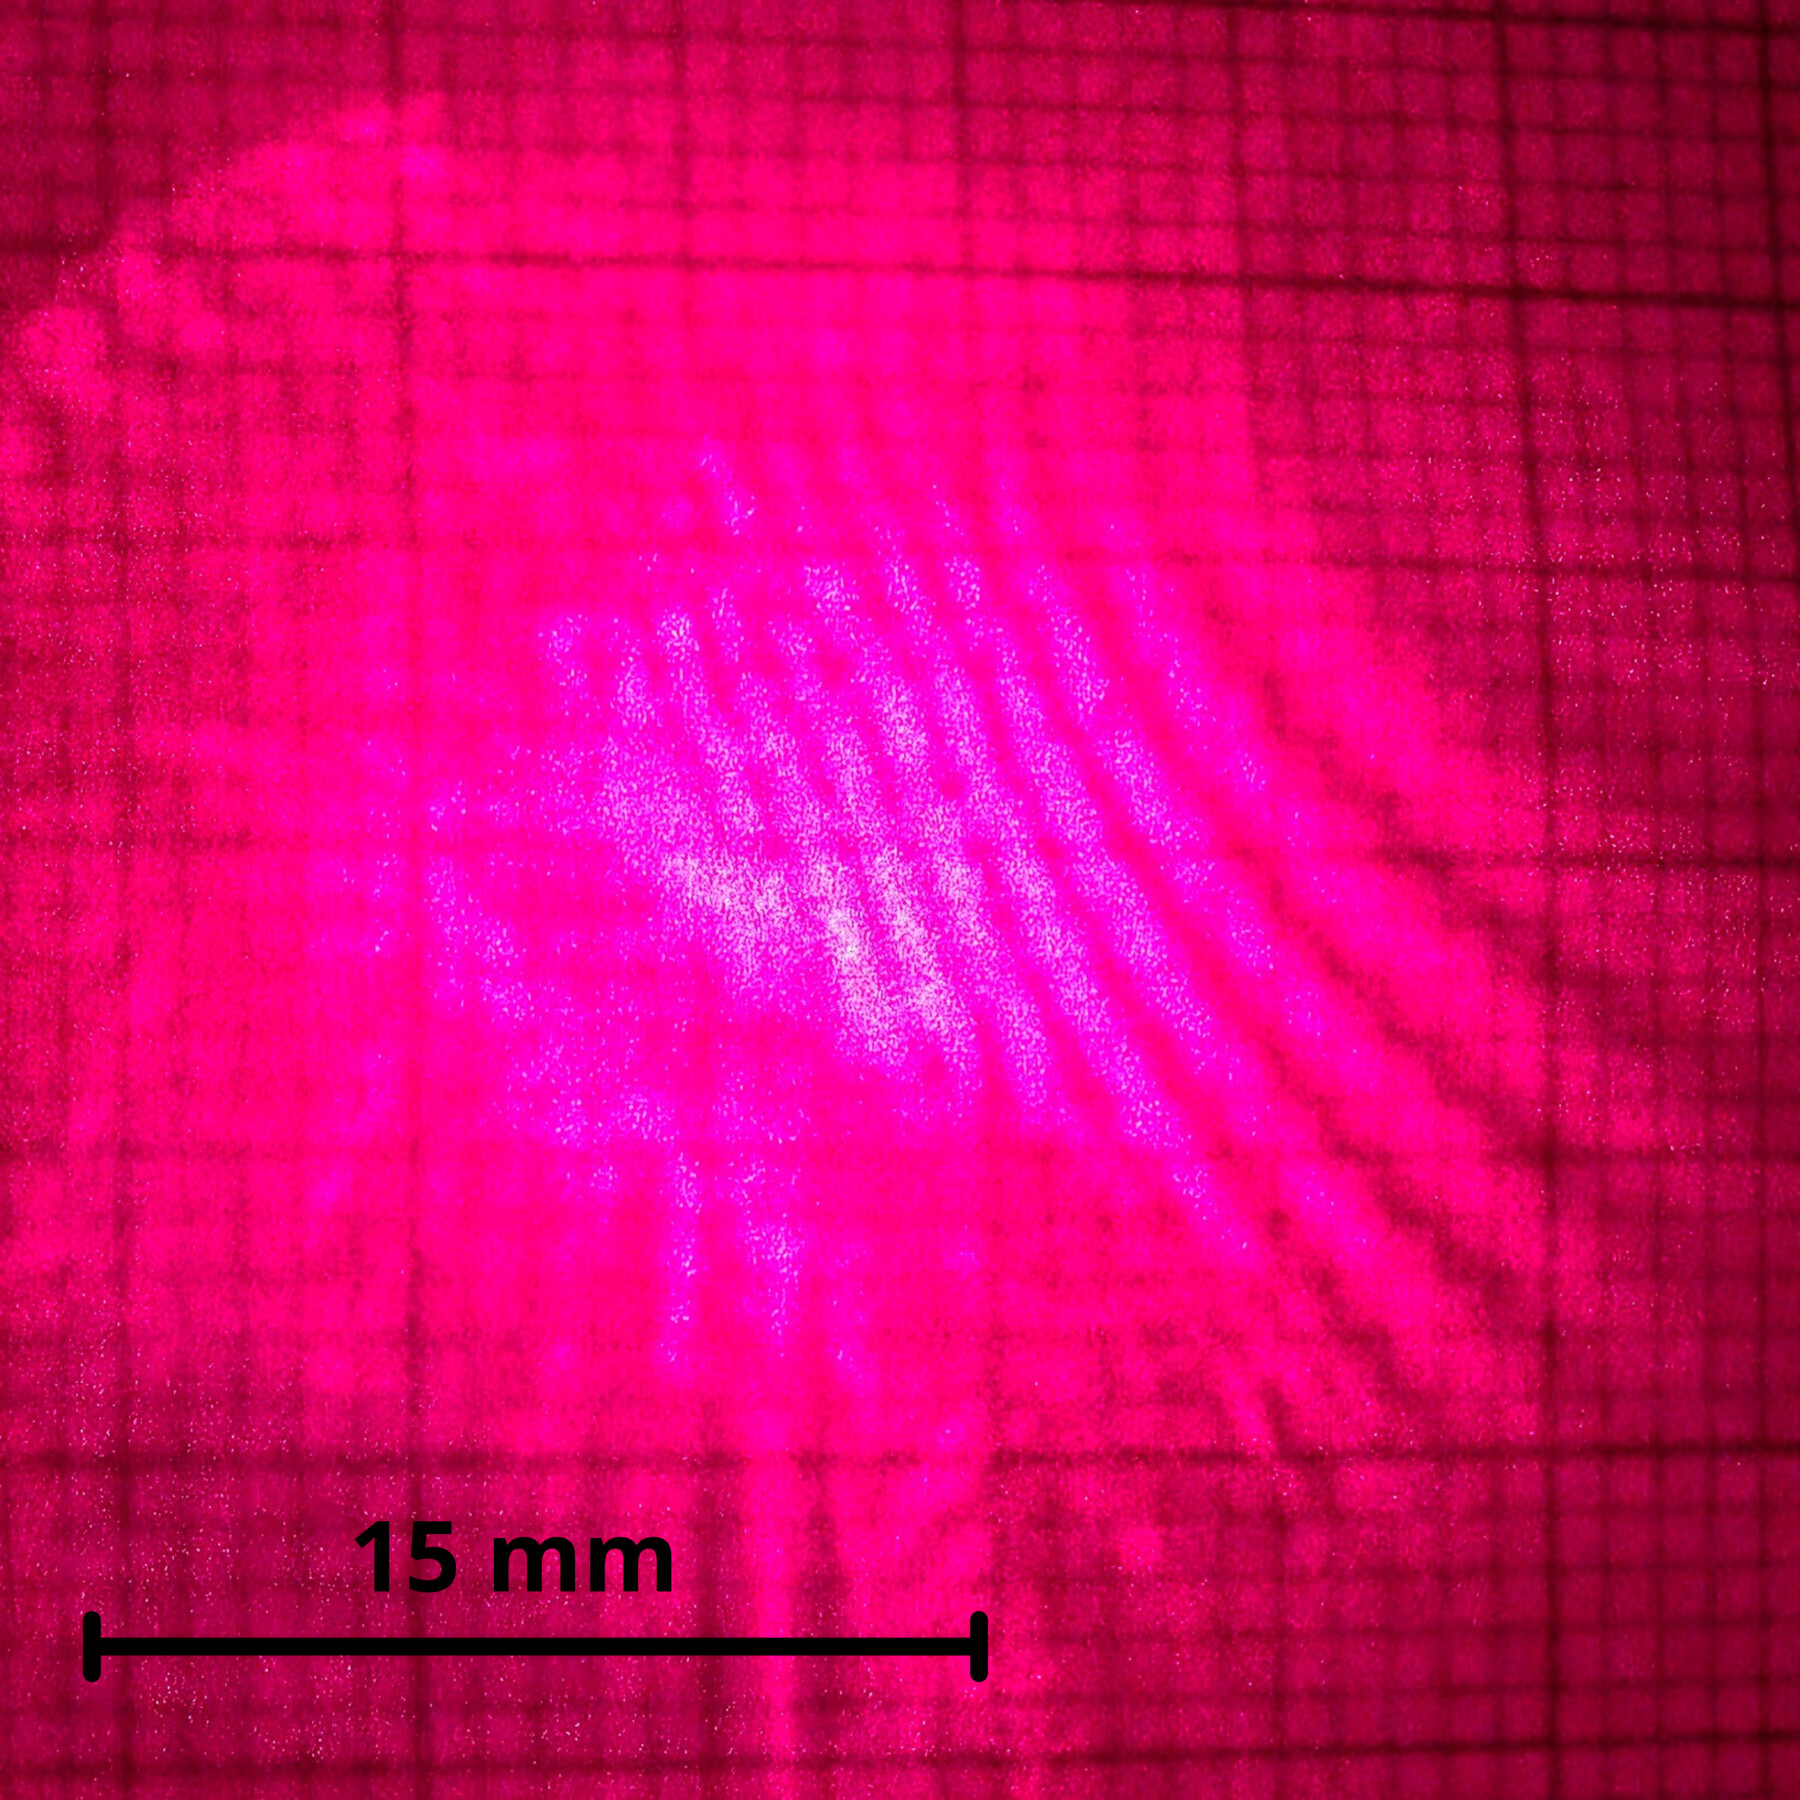
\includegraphics[width=\textwidth]{images/pattern_2mm_back_compressed.jpg}
        \caption{Pattern 2mm}
        \label{fig:pattern_2mm_back_a}
    \end{subfigure}\hfill
    \begin{subfigure}{0.45\textwidth}
        \centering
        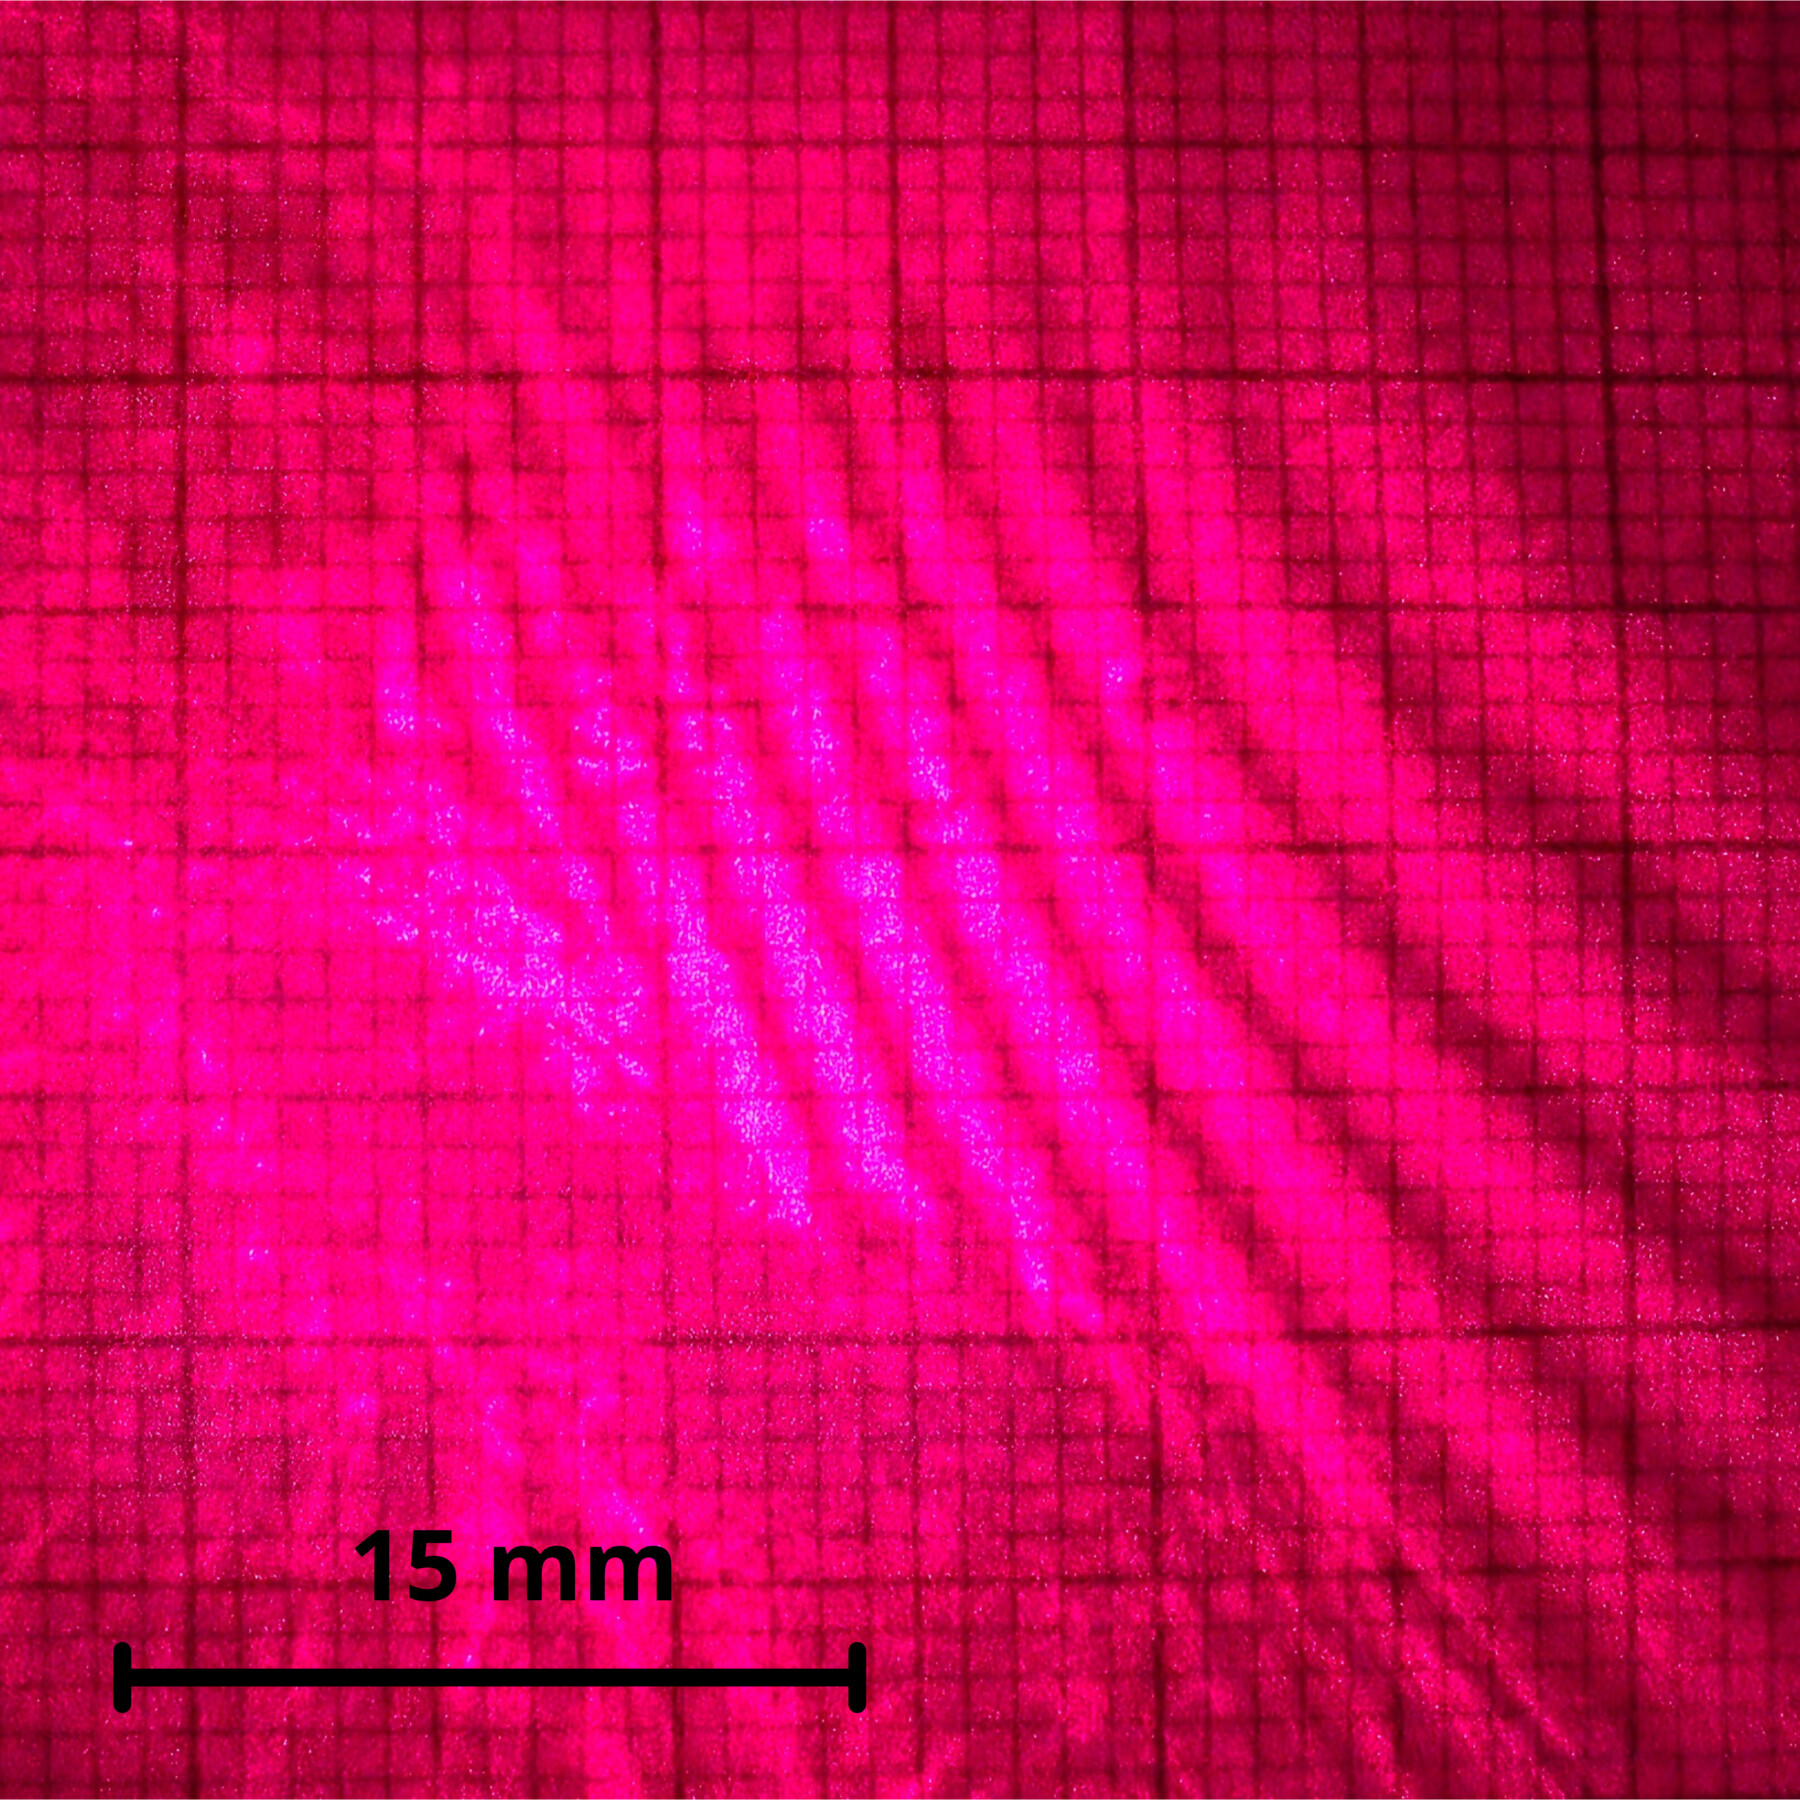
\includegraphics[width=\textwidth]{images/pattern_4mm_back_compressed.jpg}
        \caption{Pattern 4mm}
        \label{fig:pattern_2mm_back_b}
    \end{subfigure}
    \caption{Interference pattern obtained from the interferometer through a piece of paper as objective. a) Interferometer at 2 mm of the objective; b) Interferometer at 4 mm of the objective.}
    \label{fig:patterns_back}
\end{figure}
